\documentclass{article}
\usepackage[utf8]{inputenc}
\usepackage[T1]{fontenc}
\usepackage{lmodern}
\usepackage[cm]{fullpage} %very small margins (around 1.5cm)
\usepackage{enumitem} %remove vertical space in itemize with: [noitemsep,nolistsep]
\usepackage{multicol} %use \begin{multicols}{#} for # columns 
\usepackage{graphicx} %use \includegraphics[scale=1.00]{file.jpg} for images
\usepackage{color}
\usepackage[usenames,dvipsnames]{xcolor}
\usepackage{lastpage} %page x of y with: \cfoot{\thepage{} of \pageref{LastPage}}
\usepackage{fancyhdr} % also needed for footers
\usepackage{minted} %use \begin{minted}[mathescape,linenos,numbersep=5pt,gobble=0,framesep=2mm]{c++}

\fancyhead{}
\fancyfoot{}
\lfoot{\textcolor{gray}{M.Bysiek R.Łojek S.Peryt}}
\cfoot{page \thepage{} of \pageref{LastPage}}
\rfoot{\textcolor{gray}{VaDoR}}
\pagestyle{fancy}
\renewcommand{\headrulewidth}{0pt}
\renewcommand{\footrulewidth}{0pt}

\begin{document}

\title{VAnishing DOmino pRoblem - VaDoR}
\author{Mateusz Bysiek, Radosław Łojek, Stanisław Peryt; Computer Science, MiNI, WUT}
\date{21 November 2012}
\maketitle

\begin{multicols}{2}
\begin{flushleft}

\includegraphics[scale=0.60]{logo_pw.jpg}
\end{flushleft}
\begin{flushright}

\includegraphics[scale=0.25]{logo_mini.png}
\end{flushright}
\end{multicols}

\tableofcontents

\pagebreak[4]

\section{Problem description}
Vanishing domino problem. Full definition is available in the document provided by laboratories
supervisor. From now on, the problem will be referred to as VaDoR.


\section{Description of the input/output formats}

\subsection{Input}
\subsubsection{Text file}
Described in the documentation provided by the laboratories supervisor.

\subsubsection{Our own format}
XML file.
\begin{minted}[linenos,numbersep=5pt]{xml}
<domino_board width="5" height="4">
    <piece x="0" y="0" orientation="vertical" value1="2" value2="1" />
    <piece x="0" y="2" orientation="vertical" value1="3" value2="2" />
    <piece x="1" y="0" orientation="horizontal" value1="1" value2="0" />
    <piece x="1" y="1" orientation="vertical" value1="3" value2="0" />
    <piece x="1" y="3" orientation="horizontal" value1="0" value2="0" />
    <piece x="2" y="1" orientation="vertical" value1="1" value2="1" />
    <piece x="3" y="0" orientation="horizontal" value1="3" value2="3" />
    <piece x="3" y="1" orientation="vertical" value1="0" value2="2" />
    <piece x="3" y="3" orientation="horizontal" value1="2" value2="2" />
    <piece x="4" y="1" orientation="vertical" value1="4" value2="4" />
</domino_board>
\end{minted}

\noindent Description of the \verb|piece| tag:
\begin{itemize}[noitemsep,nolistsep]
  \item x - coordinate, from zero, increasing from the right to the left side of the board
  \item y - coordinate, from zero, increasing from the top to the bottom side of the board
  \item orientation:
   \begin{itemize}[noitemsep,nolistsep]
   \item \emph{horizontal} - the piece starts at $(x,y)$ and ends at $(x+1,y)$
   \item \emph{vertical} - the piece starts at $(x,y)$ and ends at $(x,y+1)$
   \end{itemize}
  \item value1 - value of the beginning of the piece i.e. value at $(x,y)$
  \item value2 - value of the end of the piece i.e. location depends on the orientation
\end{itemize}

\vspace{10pt}

If a tag \verb|removed_pieces| is present inside the \verb|domino_board| tag, it is ignored. If an
attribute \verb|order| is attached to the \verb|piece| tag, it is also ignored. That way the output file 
can be used as an input, and pieces can be rearanged and put back on the board using a text editor, without
worrying about problems with parsing.


\subsection{Output}
% Another XML file.
% 
% \begin{minted}[linenos,numbersep=5pt]{xml}
% <domino_board width="5" height="4">
%     <piece x="0" y="0" orientation="vertical" value1="2" value2="1" />
%     <piece x="0" y="2" orientation="vertical" value1="3" value2="2" />
%     <piece x="3" y="0" orientation="horizontal" value1="3" value2="3" />
%     <piece x="4" y="1" orientation="vertical" value1="4" value2="4" />
%     <removed_pieces>
%        <piece order="0" x="1" y="0" orientation="horizontal" value1="1" value2="0" />
%        <piece order="1" x="1" y="1" orientation="vertical" value1="3" value2="0" />
%        <piece order="2" x="2" y="1" orientation="vertical" value1="1" value2="1" />
%        <piece order="3" x="3" y="1" orientation="vertical" value1="0" value2="2" />
%        <piece order="4" x="1" y="3" orientation="horizontal" value1="0" value2="0" />
%        <piece order="5" x="3" y="3" orientation="horizontal" value1="2" value2="2" />
%     </removed_pieces>
% </domino_board>
% \end{minted}
% 
% It is an extension of an input format. Program will be designed in such a way, that output from the program 
% can be used again as an input (as it is described in ``Input'' section).
% 
% \vspace{7pt}
% 
% Description of extension the \verb|piece| tag:
% \begin{itemize}[noitemsep,nolistsep]
%   \item order - number, from zero, increasing in order in which the pieces were removed from the board
% \end{itemize}
% 
% \vspace{7pt}
% 
% The \verb|removed_pieces| tag contains all of the pieces that were removed from the board, with complete 
% information about their origin. 

Output is given either as output in command line, or as a graphical representation of a final state
of the board in GUI. Output format depends on how user launched the application.


\pagebreak[4]

\section{Description of the accurate algorithm}
\subsection{Class variables}
Main class of the program is called domino\_problem. Rough list of fields of the class:

\begin{minted}[linenos,numbersep=5pt]{ruby}
# size_t is an integral type
# elements_t is a list of domino pieces
# board_t is a two-dimensional array of references to the halves of domino pieces
   size_t width
   size_t height
   # collection of pieces
   elements_t elements
   # collection of halves of pieces that come from 'elements' field
   board_t board
   # pieces currently on the board
   elements_t on_board
   # possible to remove in the next turn
   elements_t possible
   # not longer on board, removed in the previous turns
   elements_t removed
   # algorithm does not know anything about these pieces
   elements_t unresolved
   # possible to remove if other pieces are placed right
   elements_t checked
   # impossible to remove due to size of the board and/or dependencies on other invalid pieces
   elements_t invalid
\end{minted}

There is also a derived class, called domino\_problem\_solver, which contains several other
variables, which store data about every state analyzed by the algorithm.

\begin{minted}[mathescape,linenos,numbersep=5pt,gobble=0,framesep=2mm]{ruby}
# state_list_t is a list of states (domino_problem-s)
# dag_t is a directed acyclic graph
# hash_t is a radix-based hashing table for integral types
   # contains unexplored states
   state_list_t unexplored
   # contains current tree of states (some explored, some not) connected
   #  according to the rules given below
   dag_t tree
   # contains explored states
   hash_t hashed
   # reference to currently best known state (state with max. number of removed pieces)
   domino_problem best_state
\end{minted}

%\pagebreak[4]

\subsection{Algorithm}
%Because of large number of loops involved in the algorithm, 
%I will provide pseudo-code, and will write down 
%a description of instructions.
% \begin{enumerate}[noitemsep,nolistsep]
%    \item Input data is read: width and height.
%    \item All pieces present on board are stored into 'elements' field
%    this list does not change with time
%    \item 'board' is generated for convienience.
%    \item 'elements' are copied into other lists: 'on\_board' and 'unresolved'
%    \item 'unresolved' are partitioned into 'checked' and 'invalid'
%    \item add current problem to the graph
%    \item CHECKING: each piece from 'checked' is examined, and if it can be removed 
%    from the board it is copied to 'possible'
%    \item for each 'possible' piece, new object of class domino\_problem is created
%    via copy constructor
%    \begin{enumerate}[noitemsep,nolistsep]
%       \item from each copy of current domino\_problem, the corresponding piece of 'possible'
%       is moved to 'removed', and the same piece is deleted from 'checked', 'on\_board' 
%       and 'board'.
%       \item all lists of 'possible' from current domino\_problem copies are cleared
%       \item add all copies to the graph with exception of those that already exist
%       in the graph, because removing first piece A and then B gives the same resulting state 
%       as removing first piece B and then A. Calculating all possibilities with duplicates would
%       result in factorial complexity of the algorithm ($n!$).
%       \item connect current problem to all of the copies
%       \item for each copy, perform all steps starting from CHECKING
%    \end{enumerate}
%    \item after the graph is constructed, find the longest path, starting from 
%    initial domino\_problem.
% \end{enumerate}

Below is an outline of the algorithm for deterministic RAM:

\begin{minted}[linenos,numbersep=5pt]{ruby}
   # 1. read input data
   width = from input
   height = from input
   elements = all pieces present on board # this list does not change with time
   # board is generated using 3 above variables
   board = generate_board(elements, width, height) 
   # 'elements' are copied into 'on_board' and 'unresolved'
   on_board = unresolved = elements
   # 'unresolved' are partitioned into 'checked' and 'invalid'
   resolve(unresolved, checked, invalid)
   # current state is copied from initial data of the problem, and it is put into the tree,
   #  becoming its root
   domino_problem current_state = self
   tree += current_state
   unexplored += current_state
   best_state = current_state
   # all pieces that can be removed in current state are found,
   #  by analyzing the 'checked' list
   find_possible(current_state)
   
   # 2. build the tree of states
   while unexplored is not empty do
      domino_problem s = unexplored.last_element
      unexplored -= s
      
      state_list_t new_states
      for element e in s.possible
         # make a copy of 's', with the exception of list of possible pieces
         domino_problem pr = s 
         # from copy of current domino\_problem, the corresponding piece is added to 'removed',
         # and the same piece is deleted from 'checked' and 'on\_board'
         pr.on_board -= e
         pr.checked -= e
         pr.removed += e
         find_possible(pr)
         new_states += pr
      end
       
      # sort new_states ascending, using length of list of 'possible' as criteria
      sort(new_states)
      
      # add all new states to 'tree', with exception of those that already exist
      # in 'tree', because removing first piece A and then B gives the same resulting state 
      # as removing first piece B and then A. Calculating all possibilities with duplicates would
      # result in factorial complexity of the algorithm (n!).
      for domino_problem st in new_states
         if hashed does not contain st
            hashed += st
            unexplored += st
            # add the new state to 'tree', as a child of 's'
            add_child(tree, s, st)
         end
      end
      
      if best_state.on_board.length > s.on_board.length then
         best_state = s
         if best_state.on_board.length == invalid.length then
            break
      end
   
      # this optimization causes complexity to go beyond 2^n, but it is used only if
      # algorithm would have ended computation otherwise due to no memory
      if running out of memory then
         hashed.remove_all
      end
   end
   
   # 3. return final result
   return best_state
\end{minted}

\subsection{Estimation of complexity}

\subsubsection{Number of states}
Let us assume that we have a set of $n$ domino pieces that are arranged on a board. Then, 
let us assume that we are taking away pieces from the board, one at a time. If we consider each 
state after removing a piece, how many different states do we have? For a given state, for each piece, 
we have a choice: the piece either is on the board, or it is not. In total we have $2$ possible scenarios
for one piece, and $n$ pieces, which gives us exactly $2^n$ different states.

\subsubsection{Relations between the states}
We can construct a following directed acyclic graph (DAG) $G$:
\begin{enumerate}[noitemsep,nolistsep]
  \item each vertex $V$ represents a state (configuration of pieces on the board)
  \item each directed edge $E$ represents the relation between states. Edges 
  are positioned in such way, that start point is at state $V_1$, and such that 
  the end point of the edge is connected to the state $V_2$ that can be obtained 
  directly from state $V_1$ by removing one domino piece from the board.
\end{enumerate}

\subsubsection{Proof that VaDoR is NP}

Below, outline of a polynomial-time algorithm for a non-deterministic RAM:

\begin{minted}[linenos,numbersep=5pt]{ruby}
input: b # list of elements on board

var r # list of removed elements, initially empty

for each element e in b
   # magical 'if' that knows when putting current element to the list 
   #  is the best possible option - such 'if-better' is allowed for non. det. RAMs
   if-better 
      add e to r
   else
      next

return r

\end{minted}

\subsubsection{Final estimation of complexity}
Having a DAG $G$, the domino problem is equivalent to finding the longest path of DAG. 
Unfortunately, graph has to be constructed at runtime, and that takes time. 

Since, for each state, the calculation of related states will be performed (and there are $2^n$
states in total) I estimate the complexity of accurate algorithm as exponential. Due to this maximum
number of states, I also informally classify this algorithm as NP-complete, however, it is only my
intuition.

After the DAG is constructed, by finding its longest path, an optimal solution is obtained. But,
because the DAG is not given as input, but rather constructed during algorithm's operation, finding
longest path can be done while constructing the DAG, therefore no extra time is needed for it.

My estimations indicate that calculation of possible sub-states for a given single state takes
polynomial time. Therefore, the total complexity of the accurate algorithm should be roughly $ 2^n $
In practice, however, I have noticed that it is not such, because problems encountered in practice
tend to have far less possible choices, due to strong inter-piece dependencies.
 

\section{Description of the approximate algorithms}

\subsection{Approximation by Mateusz Bysiek}

\subsubsection{Class variables}
The same as in case of accurate algorithm.

\subsubsection{Algorithm}
Development of approximations of NP problems is usually a consequence 
of deep understanding of the problem, and extensive experience in solving it using
some kind of accurate algorithm.

During my experiments, I have discovered that depth-first construction/search of DAG is far more
efficient than breadth-first, when it comes to actual time needed to find the best result. It is so
because we need to find any best result, not all of them. In case of breadth-first, 

I have put all above optimizations into the accurate algorithm, and I have created approximate one
by simply limiting number of possible options to be explored. I have limited number of explored
options to $n^2$, where $n$ is number of elements initially on board. In short, after line 60, I
added this:

\begin{minted}[linenos,numbersep=5pt]{ruby}
   if hashed.element_count > square(elements.length)
      break
\end{minted}

\subsubsection{Optimizations}
I have also noticed that when I use depth-first search in such way as described in the accurate
algorithm's pseudo-code, the tree is searched from 'right' to 'left', and when algorithm is
analyzing any state x, that means that all states to the right of it are already explored.

I have used this to develop optimization which removes obsolete explored branches, i.e. those
branches that do not contain currently known best state. This greatly reduced memory usage.

I have also noticed that list of pieces currently on board can be easily converted to integral type
(if number of pieces initially on board is less than maximum number of bits stored in that type).
Keeping all lists of pieces (with exception of the 'reference' list used to convert them back) as
integers also greatly decreased memory usage, and allowed creation of a very cheap (in terms of time
and memory) hash table (used as the field 'hashed'), which has constant access/storage/search time
equal to $\log (k)$ where $k$ is number of pieces initially on board.

The above (and some other, minor) optimizations caused the algorithm to be able to solve problems
with at most 64 not-invalid pieces. This means that if length of 'checked' exceeds 64, the program
will crash, when either accurate algorithm, or approximate algorithm created by me (M. Bysiek) is used.

\subsubsection{Complexity}
Due to hard limit of checking at most $n^2$ states, and assuming that checking each state takes
polynomial time, such approximate algorithm is also polynomial.


\pagebreak[4]

\subsection{by Stanislaw Peryt}

\subsubsection{Input Data}
collection of domino pieces from input file
\subsubsection{Description and Class Variables}
This algorithm is based on the idea of Greedy algorithms. I assume some additional classification
which is done only once for each element. For classification purposes each dominoPiece should
contain some additional fields:

\begin{minted}[linenos,numbersep=5pt]{c++}
boolean isIndependent; //can be removed even from empty board, so it does not have to 
   // be removed immediately
boolean canBeRemoved; //initially false. Changes to true, when fulfills removal conditions
list<waitingFor>; // list of pieces for which it is waiting;
list<waitForMe>; // list of pieces waiting for it;
\end{minted}

I decided to add this classification, because in greedy strategy, we could remove pieces immediately
when they fulfill removal requirements. But it may happen, that there are some pieces, for which
pieces we already removed are necessary to fulfill removal requirements. When we have this
classification based on scopes of domino pieces, we can wait with removing, and eliminate at least
some of those situations described above, providing better local optimal choices.

For this algorithm we also need:
board – contains all domino pieces that have remained on the board
roots – contains possible starting pieces, i.e. containing zero
neighbors – contains domino pieces, which are neighbors of deleted piece, i.e. pieces alongside empty fields
\subsubsection{Algorithm}
\begin{enumerate}[noitemsep,nolistsep]
   \item Create board from input
   \item Find possible roots and assign them to neighbors
   \item for each dominoPiece in board assign scopes and waiting property
   \begin{enumerate}[noitemsep,nolistsep]
      \item determine scopes based on numbers given on dominoPiece
      \item determine dominoPieces on scopes and assign them to the waitForMe list
      \item tell those pieces to assign this dominoPiece on their waitingFor list
   \end{enumerate}
   \item stop=false;
   \item while(!stop)\{
   \begin{itemize}[noitemsep,nolistsep]
     \item for each dominoPiece in neighbors\{
         \begin{enumerate}[noitemsep,nolistsep]
            \item if dominoPiece can be removed \{
            \begin{enumerate}[noitemsep,nolistsep]
               \item if (domino Piece isIndependent) and (list of pieces it is waiting for is not empty) \{ \\
                  wait with removal; \\
               \}
               \item else
                  remove it(from neighbors and board) and tell waiting pieces, if there were any waiting
                  for this piece, that it does not need waiting any more. (i.e. delete piece from waiting
                  list)
            \end{enumerate}
            \}
         \end{enumerate}
         \} \\
         determine new neighbors into temp (each removed piece can produce at most 6 new neighbors)
     \item if temp equals neighbors\{
         \begin{itemize}[noitemsep,nolistsep]
            \item check if (something can be removed): remove first;
            \item else stop=true;
         \end{itemize}
         \}
     \item else neighbors=temp;
   \end{itemize}
   \}
   \item calculate score
\end{enumerate}
\subsubsection{Estimation of complexity}
Partial Complexities:

$n$-complexity of classification

$n^2$-complexity of part at “while(!stop) loop”

In order to associate attributes for classification we need to iterate once through whole collection
which is of size n. Then in the while loop we are trying to remove pieces. In worst case we delete
only one piece in one iteration which gives us at most n runs of while and inside while loop, we
iterate through neighbors collection which is always smaller than n, but it is n dependent.
Therefore for each n, algorithm executes number of operations proportional to n, which gives us
quadratic time complexity.

Final worst case complexity : $n^2 + n$


\subsection{Approximation by Radosław Łojek}

\subsubsection{Introduction}
The solution I have designed is the most intuitive and straight forward algorithm. It checks all
possible elements along its way. If a domino piece satisfies necessary conditions of being removed,
it is thrown away from a board of elements. The operation is repeated for all consecutive elements
until nothing can't be removed, or the domino board is empty.

\subsubsection{Data structure}
The data structure I have decided to use is a two dimensional array of objects, where object is a
single domino field. Each object consists of fields such as: its value, location X and Y, boolean
saying if a piece is placed horizontally/vertically, boolean saying if it is successor or
predecessor field (value above or on the left side of a domino piece is successor, otherwise
predecessor) and of course pointer to the other half of the piece. If a single cell in a matrix is
empty, meaning that no piece is there, it is marked as a null pointer.
\\
\begin{minted}[linenos,numbersep=5pt]{c++}
class dominoField {
   int value;
   int X;
   int Y; 
   boolean isSuccessor;
   boolean isVertical; 
   dominoField *twinField; 
}
\end{minted}


\subsubsection{Algorithm Pseudo-Code}
The algorithm takes as a parameters two dimensional array of elements and its vertical and
horizontal size. Returns elements that were removed during the calculations. Below algorithm is
simple, since it does not involve more complicated concepts such as Artificial Intelligence or
complex graph algorithms.
\\
\begin{minted}[linenos,numbersep=5pt]{c++}
List<dominoPiece> solveDominoProblem(dominoField **board, int dimX, int dimY){
   List<dominoPiece> result_list;
   int iterPiecesRemoved = 1;
   
   while iterPiecesRemoved != 0 {
      iterPiecesRemoved = 0;
      for i = 0 to dimX {
         for j = 0 to dimY {
            if !isEmpty(board,i,j) and isElemRemovable(board, dimX, dimY, i, j){ 
               result_list.add( removePiece(board,i,j) );
               iterPiecesRemoved = iterPiecesRemoved + 1;
            }
         }
      }
   }
   return result_list;
}
\end{minted}

%\begin{wrapfigure}{r}{0.3\textwidth}
%  \vspace{-30pt}
  \begin{center}
    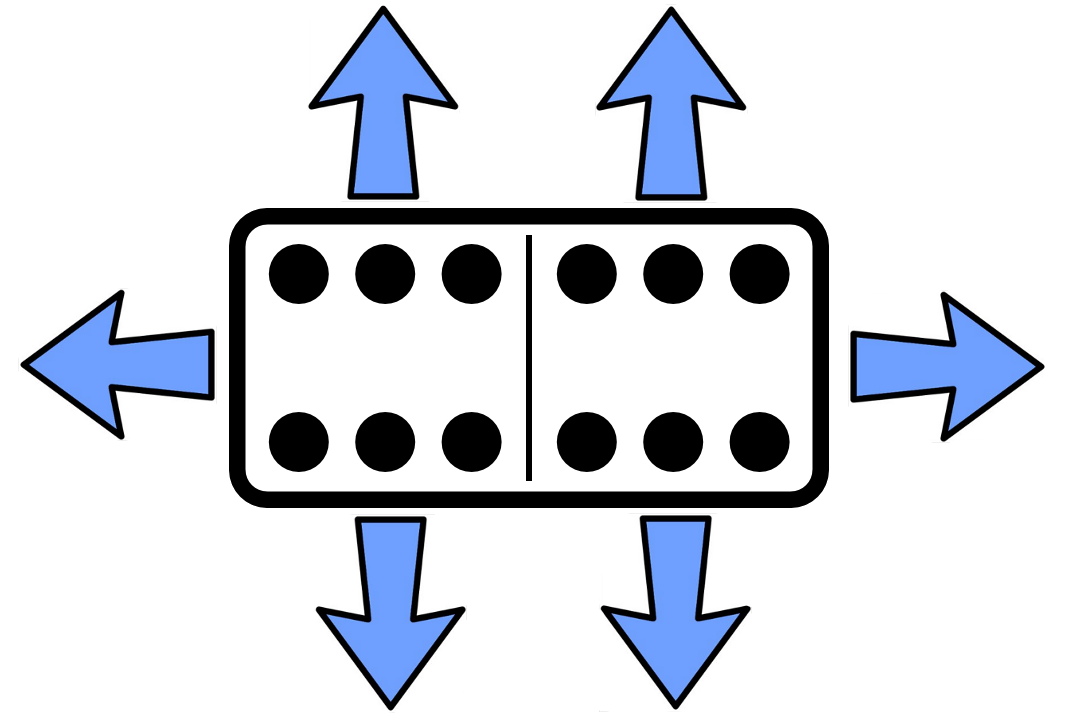
\includegraphics[width=0.2\textwidth]{dirPiece.png}
  \end{center}
 % \vspace{-20pt}
%\end{wrapfigure}

I will let myself omit pseudo code of functions used above. Just briefly explain how isElemRemovable
will work: depending on the location of a 'twinField' of a single piece, function counts the number
of empty fields in each possible direction (as depicted on the right). Once the directions are
counted, function checks if they meet requirements for the piece to be removed - if it does, returns
true or false otherwise.

\subsubsection{Time complexity}
Time complexity of the considered algorithm is \textit{$n^2$}, since we go in each iteration 
through all possible domino fields \textit{n} times. Each iteration is repeated in worst case
\textit{1/2*n} times, because may occur situation in which only one domino element (two fields)
disappears in one \textit{while} loop iteration.

\subsubsection{Example}

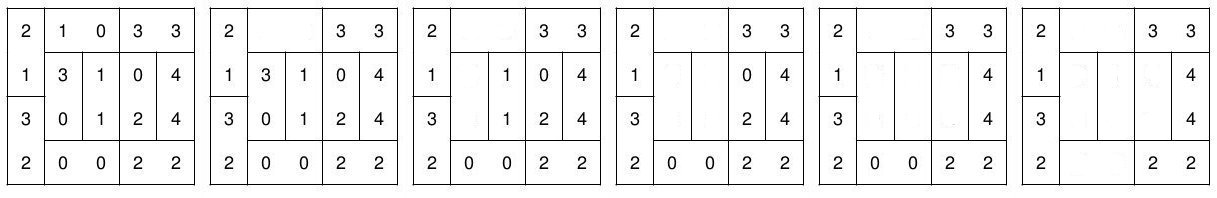
\includegraphics[width=1\textwidth]{board1.jpg} \\
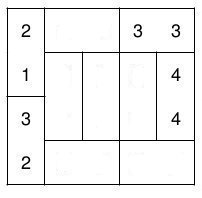
\includegraphics[width=0.163\textwidth]{board2.jpg}


\end{document}
